\begin{figure}
	%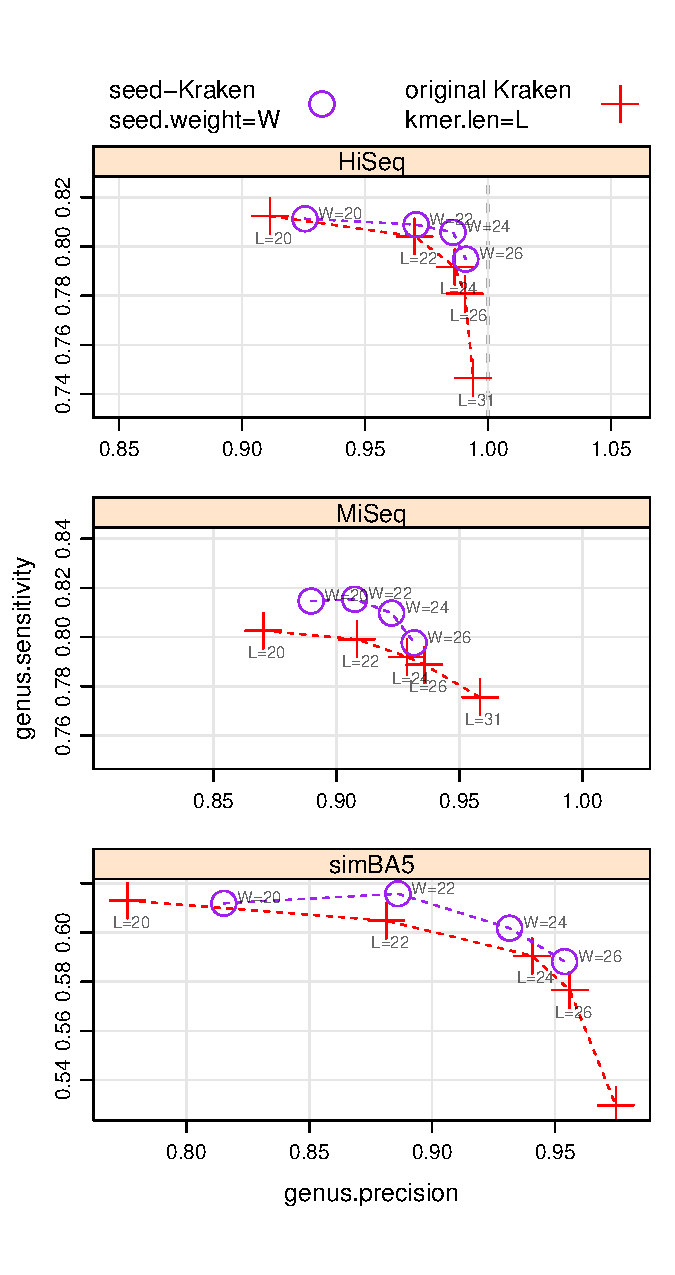
\includegraphics[width=0.5\textwidth]{images/seed-kraken_plt1_draft1.pdf}
	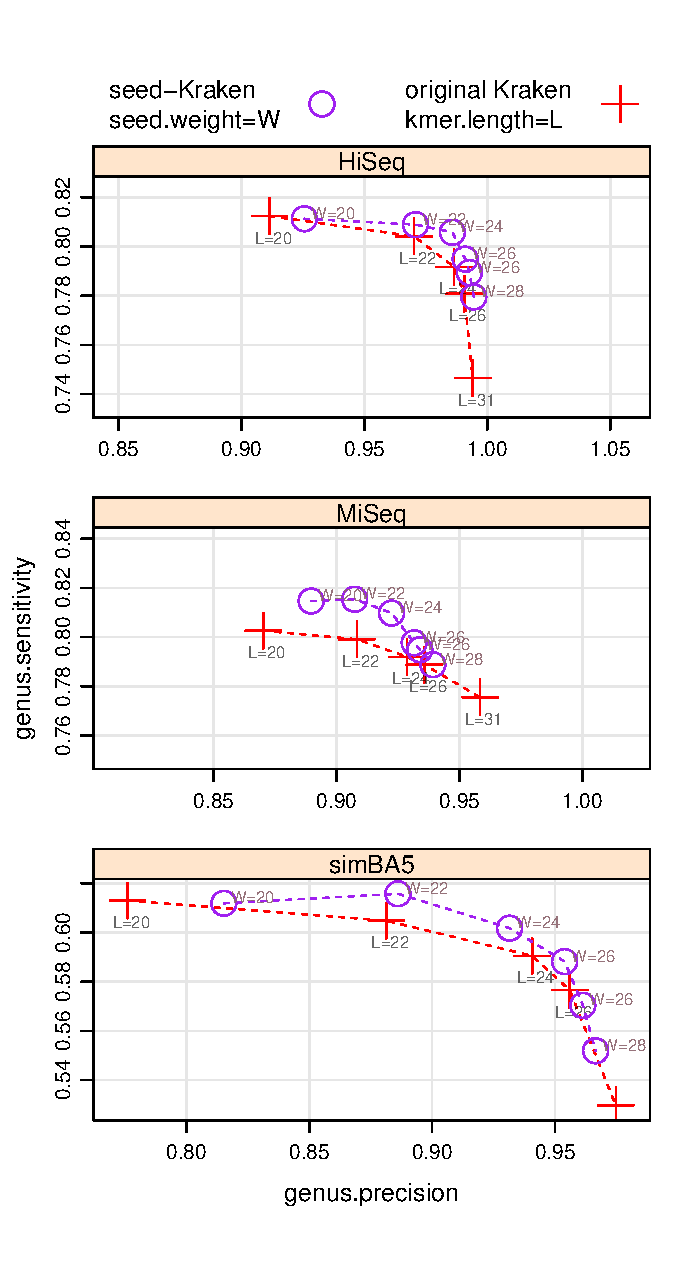
\includegraphics[width=0.5\textwidth]{images/seed-kraken_plt1_bioinfo.pdf}
	\caption{
	Classification performance of {\sc seed-Kraken} 
	and original {\sc Kraken} on three simulated metagenomes HiSeq,
% (10 bacterial genomes, low error rate), 
MiSeq 
% (10 bacterial genomes, average error rate), 
and simBA-5.
% (607 bacterial genera, high error rate). 
Charted are genus precision (positive predictive value) against genus
sensitivity (rate of correct assignments) depending on seeds, which are characterized by weights (indicated), and spans (31 to 38, not indicated). 
% Varying are $k$-mer length, and its spaced seed equivalent seed weight, while the seed span is kept constant at $31$. {\sc seed-Kraken} consistently outperforms original {\sc Kraken} in sensitivity/sensibility trade off.
	}
	\label{fig:kraken-experiments}
\end{figure}
